\documentclass[12pt]{article}
\usepackage{graphicx}
\graphicspath{ {images/} }
\usepackage[spanish]{babel}
\usepackage[utf8]{inputenc}
\usepackage[backend=biber]{biblatex}
\bibliography{ref}
\usepackage[T1]{fontenc}
\usepackage{lmodern}

\begin{document}

\thispagestyle{empty}
\begin{center}
\begin{figure}[h]
\centering

\includegraphics[width=.6\textwidth]{logo.jpg}\\
\end{figure}

\vspace{1cm}
\Large \sc  Instituto Tecnológico y de Estudios Superiores de Monterrey
\\

\vspace{2.5cm}
\Large \bf
\emph{Actividad 1. Conceptos básicos de ciencia de datos}

\vspace{2.5cm}
\Large \bf Carlos Pano Hernández\\
\vspace{0.3cm}
\Large \bf A01066264\\
\vspace{3.5cm}
\normalsize \sc \rightline{Ciencia y analítica de datos}
\vspace{0.3cm}
\normalsize \sc \rightline{Lunes 22 de Abril 2024}
\end{center}

\newpage

\section{Introducción}
En el vasto universo de la Ciencia de Datos, podemos encontrar disciplinas que emplean una amplia gama de algoritmos y técnicas para la extracción de patrones y tendencias difíciles de identificar por un humano. Desde la invención del computador de Turín en 1936 (que marcó el inicio de la era digital), hasta el explosivo crecimiento del \emph{Internet de las Cosas (IoT)}, en los últimos 20 años, hemos sido testigos de una avalancha de datos masivos de todo tipo.\\

Dentro de este orden de ideas, los grandes corporativos se encuentran con complejos sets de información que, si se analizan adecuadamente, pueden ofrecer insights poderosos para impulsar la toma de decisiones informadas y estratégicas.\\

La Ciencia de Datos, emerge como una solución entre la información en bruto y el conocimiento entendible por nosotros. Se nutre de técnicas y herramientas provenientes de sub-campos como el: \emph{aprendizaje automático}, \emph{la minería de datos}, \emph{big data} y \emph{la analítica de datos} para extraer, procesar y visualizar información de manera efectiva y significativa. En los párrafos siguientes, exploraremos con mayor profundidad estos conceptos fundamentales.\\

\section{Aprendizaje automático}
De acuerdo con Kelleher \cite{1}, el Aprendizaje Automático o comúnmente conocido como: \emph{Machine Learning}, se centra en el diseño y evaluación de algoritmos para la extracción de patrones provenientes de un conjunto de información. Dichos algoritmos (modelos) tienen la capacidad de aprender y mejorar automáticamente a partir de la experiencia. Son entrenados y construidos con bases de datos de gran magnitud para la predicción de algún valor con base a experiencia pasada. Se busca tener insights específicos.\\

Cabe destacar, que el Machine Learning es un sub-dominio de la inteligencia artificial, pues modelos como la \emph{Regresión Logística} o \emph{Regresión Lineal}, se basan en métodos matemáticos. Podemos simplificar lo anterior con el siguiente diagrama:\\

\begin{figure}[h]
\centering{
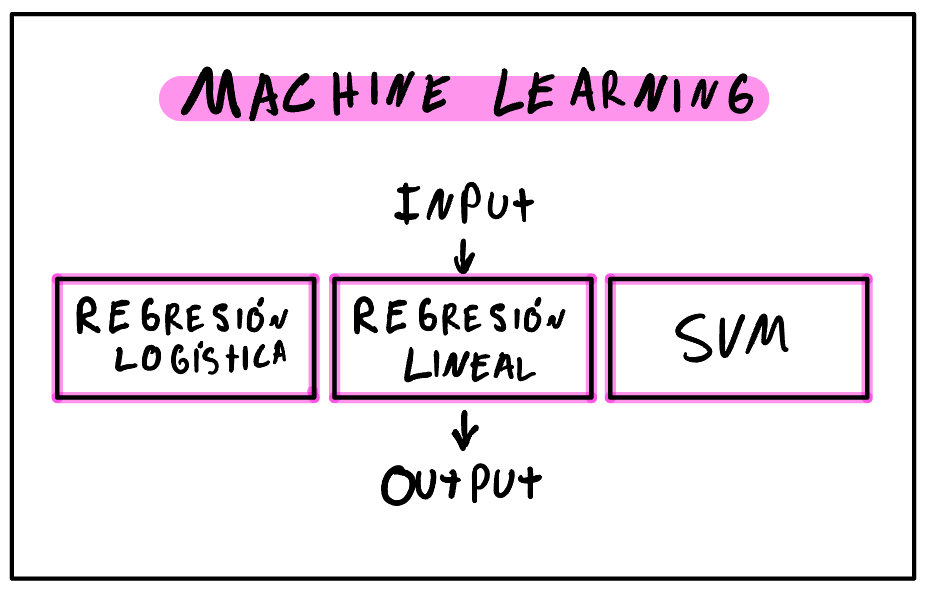
\includegraphics[width=.5\textwidth]{ML.jpeg}\\
\caption{Machine Learning overview}}
\end{figure}

\section{Minería de datos}
\emph{Data Mining}, lidia con el análisis de datos estructurados para uso comercial \cite{1}. Aquí, se filtran grandes conjuntos de datos para identificar patrones y relaciones que pueden ayudar a resolver problemas empresariales a través del análisis de datos. Las técnicas y herramientas de minería de datos ayudan a las empresas a predecir tendencias futuras y tomar decisiones empresariales más informadas.\\

\begin{figure}[h]
\centering{
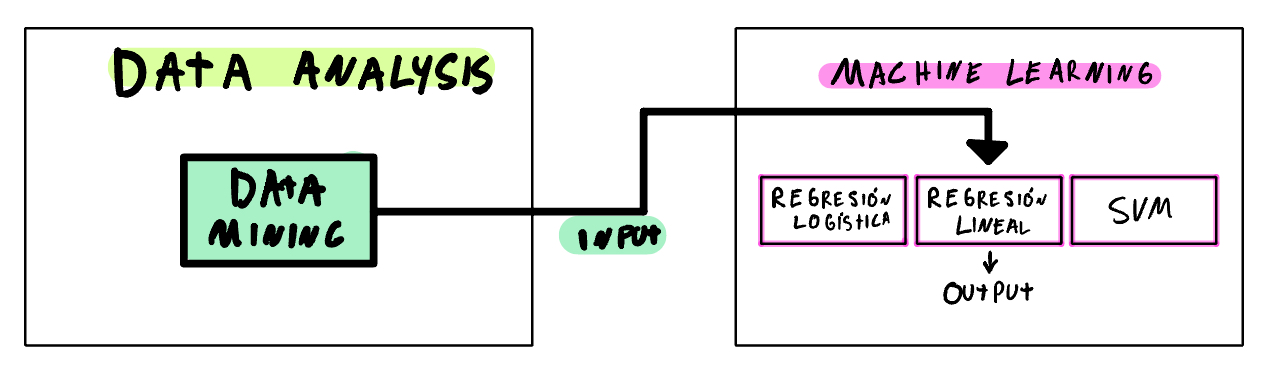
\includegraphics[width=.5\textwidth]{DM.jpeg}\\
\caption{Machine Learning overview}}
\end{figure}

\section{Big data}
Ahora bien, se presenta el concepto de Big Data. Que hace referencia misma a la cantidad de información que poseemos (Volume), los tipos de datos que componen el set de información(Variety) y la Velocidad a la que se obtienen estos datos. El concepto de \emph{Big Data} puede ser confuso en la mayoría de las veces, pues en este punto solo describe el estado mismo de la información a procesar, tal como se muestra a continuación \cite{1}.\\
\begin{figure}[h]
\centering{
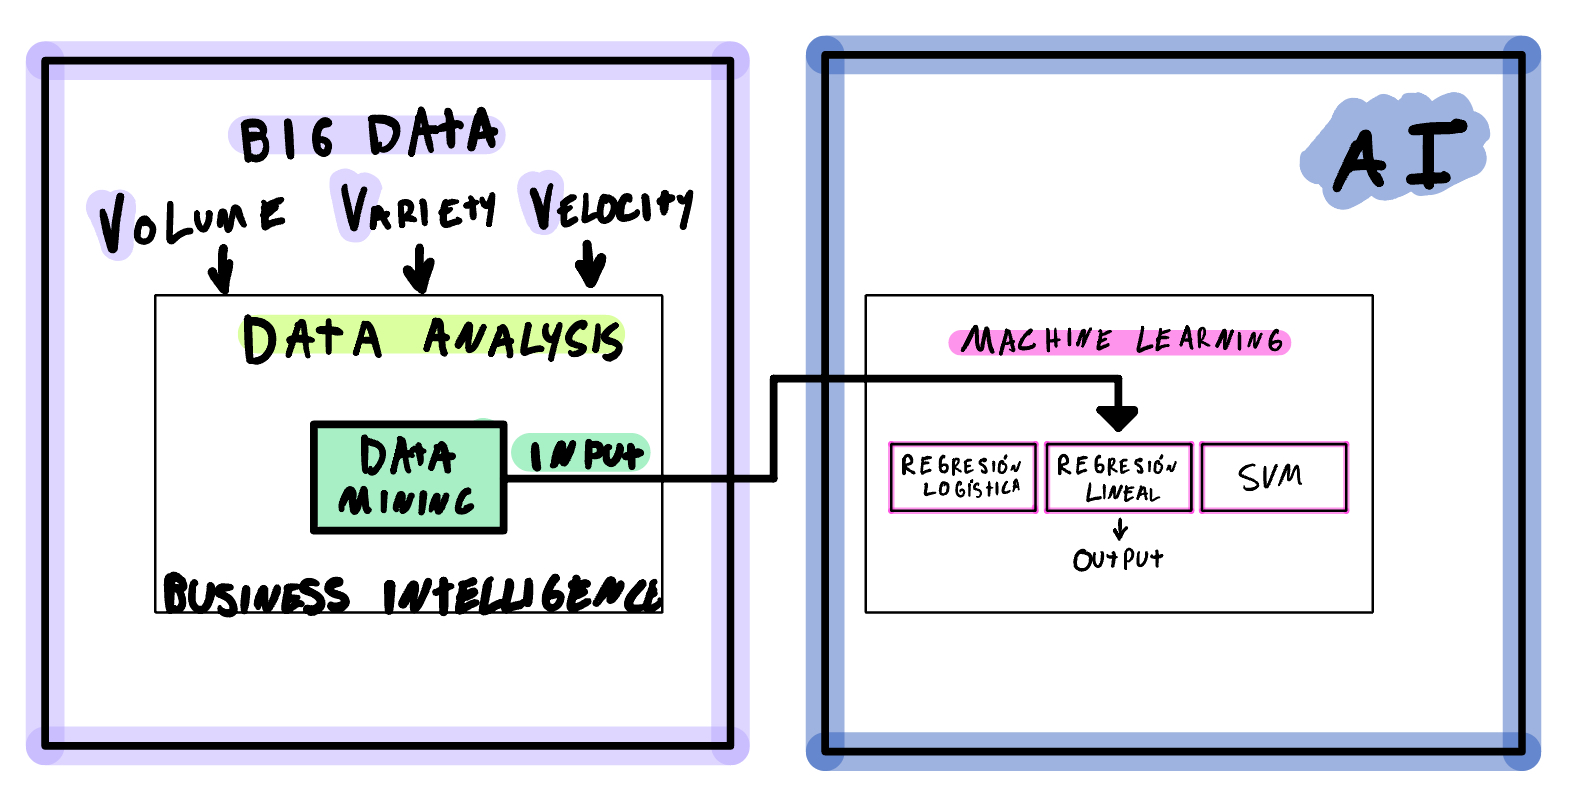
\includegraphics[width=.5\textwidth]{BD.jpeg}\\
\caption{Big Data overview}}
\end{figure}

Estos datos deben ser gestionados de la mejor manera posible, para así llegar a mejores resultados.

\section{Analítica de datos}
Como vimos en la Figura 3, la Analítica de Datos engloba la examinación, limpieaza y transformación de datos para descubrir información útil, inferir conclusiones y apoyar la toma de decisiones (Business Intelligence)\cite{1}. Incluye diversas técnicas, desde el análisis descriptivo hasta el análisis predictivo y prescriptivo.\\

\section{¿Cómo se relaciona cada uno de estos 4 elementos con la ciencia de datos?}
Con base a los conceptos anteriores, y como conclusión, vemos que estos términos forman parte pequeña de un todo en la Ciencia de Datos. Big Data es la información en crudo que se genera día con día y se califica con base a su variedad y volumen. Los científicos de datos utilizan ciertas técnicas para procesar estos sets de información, crear insights accionables y tomar decisiones en consecuencia de los mismos (Business Intelligence).\\

La minería de datos es una parte integral de la ciencia de datos. Ayuda a los científicos de datos a identificar patrones no obvios para las personas y si lo amerita, generar modelos predictivos y descriptivos (ML) para la automatización de ciertos procesos.\\

\begin{thebibliography}{a}

% Ejemplo de libro
\bibitem{kelleher18} 
Kelleher, J. D., and Tierney, B. (2018). \emph{Data science}. The MIT Press.

\end{thebibliography}

\end{document}